% Contoh penggunaan kelas prodimat
% Opsi: \documentclass[nonumsec]{prodimat} untuk menghilangkan nomor bagian
\documentclass{prodimat}

\judul{Judul Artikel dengan Maksimal 12 Kata}
\penulis{Nama Mahasiswa\textsuperscript{1,a}, Nama Dosen Pembimbing\textsuperscript{2}}
\afiliasi{1}{Mahasiswa Program Studi Matematika FST Universitas Terbuka}
\afiliasi{2}{Program Studi Matematika FST Universitas Terbuka}
\email{a}{email\_mahasiswa@ecampus.ut.ac.id}

\begin{document}
\maketitle

\begin{abstrak}
Isi abstrak terdiri dari satu paragraf dengan 150--200 kata. Abstrak memuat hasil utama dan kesimpulan penelitian, tanpa tabel, gambar, maupun daftar pustaka.
\end{abstrak}
\katakunci{graf, hipergraf, keterhubungan}

\section{Pendahuluan}
Latar belakang, perumusan masalah, dan tujuan penelitian ditulis di sini. Konsep ini digunakan antara lain pada \citet{light2008} dan \citep{wooldridge2012}.

\section{Metode}
Rumus yang diacu dalam pembahasan diberi nomor, seperti pada \eqref{eq:trig}.
\begin{equation}\label{eq:trig}
  \cos^{2}x + \sin^{2}x = 1
\end{equation}
Berdasarkan \eqref{eq:trig}, identitas trigonometri berlaku. Rumus yang tidak diacu cukup ditulis dengan \texttt{equation*}:
\begin{equation*}
  e^{i\pi} + 1 = 0
\end{equation*}

\section{Hasil dan Pembahasan}
\begin{definisi}\label{def:hipergraf}
Hipergraf $H=(X(H),E(H))$ adalah pasangan himpunan simpul $X(H)$ dan himpunan sisi $E(H)$.
\end{definisi}

\begin{lema}\label{lem:bantu}
Setiap hipergraf terhubung dengan $|E(H)|\ge 1$ memiliki paling sedikit satu sisi.
\end{lema}
\begin{proof}
Tulis bukti di sini.
\end{proof}

\begin{teorema}[Carpentier dkk., 2014]\label{teo:utama}
Misalkan $H=(X(H),E(H))$ hipergraf terhubung dengan $|E(H)|\ge 1$. Maka $H$ terhubung minimal jika dan hanya jika $rc(H)=|E(H)|$.
\end{teorema}
\begin{proof}
Tulis bukti di sini sesuai \cref{lem:bantu}.
\end{proof}

\begin{contoh}\label{cont:1}
Tulis contoh di sini.
\end{contoh}

Berdasarkan \cref{tab:jarak} dan \cref{fig:grafik}, dapat dilihat bahwa kecepatan tidak selalu meningkat terhadap jarak.

\begin{figure}[htbp]
  \centering
  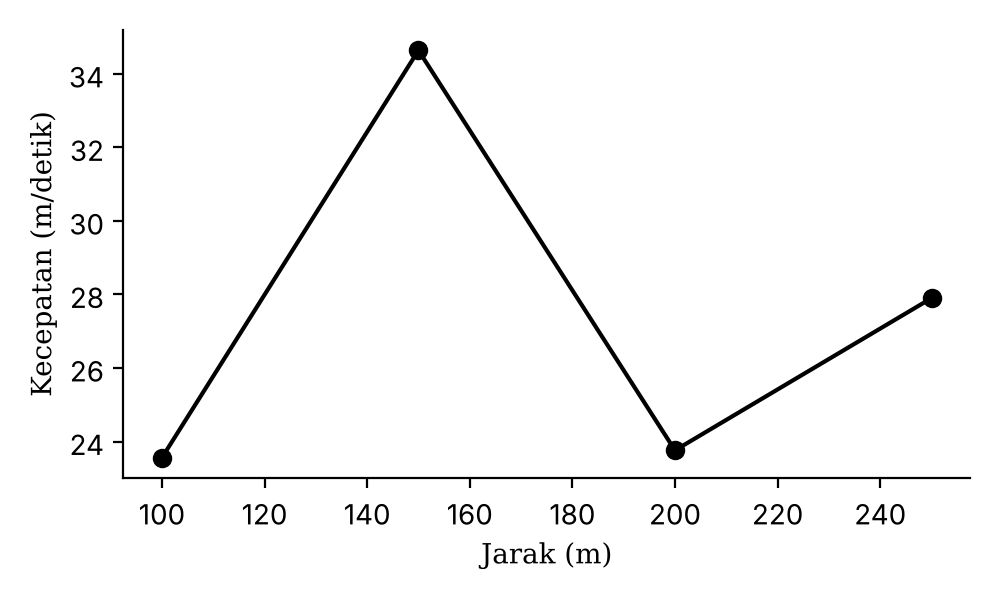
\includegraphics[width=0.6\textwidth]{contoh-grafik.png}
  \caption{Contoh grafik}
  \label{fig:grafik}
  \sumber{xys.com}
\end{figure}

\begin{table}[htbp]
  \centering
  \caption{Tabel ini adalah contoh tabel sederhana (Sumber : data diolah (2002))}
  \label{tab:jarak}
  \begin{tabular}{cc}
    \toprule
    Jarak (m) & Kecepatan (m/detik) \\
    \midrule
    100 & 23{,}56 \\
    150 & 34{,}64 \\
    200 & 23{,}76 \\
    250 & 27{,}9  \\
    \bottomrule
  \end{tabular}
\end{table}

\section{Kesimpulan}
Kesimpulan dari hasil penelitian, serta saran untuk penelitian lanjutan.

\bibliographystyle{prodimat}
\bibliography{referensi}
\end{document}
